%% LyX 2.0.5.1 c	reated this file.  For more info, see http://www.lyx.org/.
%% Do not edit unless you really know what you are doing.
\documentclass[11pt,oneside,final]{fithesis2}
%\usepackage[total={30em	,23cm}, includefoot]{geometry}

%% Basic packages
\usepackage[czech]{babel}
\usepackage{cmap}
\usepackage[T1]{fontenc}
\usepackage{lmodern}
\usepackage[utf8]{inputenc}
\usepackage{graphicx}

%% Additional packages for colors, advanced
%% formatting options, etc.
\usepackage{color}
\usepackage{microtype}
\usepackage{url}
\usepackage{cslatexquotes}
\usepackage{fancyvrb}
\usepackage[small,bf]{caption}
\usepackage[plainpages=false,pdfpagelabels,unicode]{hyperref}
\usepackage[all]{hypcap}

%% Martinovy balíky
\languageattribute{czech}{split}
\usepackage{cite}
\setcounter{secnumdepth}{3}
\setcounter{tocdepth}{3}
\usepackage{hanging}
\usepackage{listings}
\usepackage{comment}
\usepackage{textcomp}
\definecolor{listinggray}{gray}{0.9}
\definecolor{lbcolor}{rgb}{0.9,0.9,0.9}
\usepackage{zref-user}
\renewcommand{\baselinestretch}{1.13}

\newcommand\todo[1]{\noindent\textcolor{red}{#1}}
\newcommand\nove[1]{\textcolor{green}{#1}}

\lstset{
	%backgroundcolor=\color{lbcolor},
	tabsize=4,
	rulecolor=,
        basicstyle=\scriptsize,
        upquote=true,
        aboveskip={1.5\baselineskip},
        columns=fixed,
        showstringspaces=false,
        extendedchars=true,
        breaklines=true,
        prebreak = \raisebox{0ex}[0ex][0ex]{\ensuremath{\hookleftarrow}},
        frame=single,
        showtabs=false,
        captionpos=b, 
        showspaces=false,
        showstringspaces=false,
        identifierstyle=\ttfamily,
        keywordstyle=\color[rgb]{0,0,1},
        commentstyle=\color[rgb]{0.133,0.545,0.133},
        stringstyle=\color[rgb]{0.627,0.126,0.941},
        extendedchars=true,
        inputencoding=utf8,
    extendedchars=true,
    literate=%
    {á}{{\'a}}1
    {č}{{\v{c}}}1
    {ď}{{ \v{d}}}1
    {é}{{\'e}}1
    {ě}{{\v{e}}}1
    {í}{{\'i}}1
    {ň}{{\v{n}}}1
    {ó}{{\'o}}1
    {ř}{{\v{r}}}1
    {š}{{\v{s}}}1
    {ť}{{\v{t}}}1
    {ú}{{\'u}}1
    {ů}{{\r{u}}}1
    {ý}{{\'y}}1
    {ž}{{\v{z}}}1
    {Á}{{\'A}}1
    {Č}{{\v{C}}}1
    {Ď}{{\v{D}}}1
    {É}{{\'E}}1
    {Ě}{{\v{E}}}1
    {Í}{{\'I}}1
    {Ň}{{\v{N}}}1
    {Ó}{{\'O}}1
    {Ř}{{\v{R}}}1
    {Š}{{\v{S}}}1
    {Ť}{{\v{T}}}1
    {Ú}{{\'U}}1
    {Ů}{{\r{U}}}1
    {Ý}{{\'Y}}1
    {Ž}{{\v{Z}}}1   
}

\definecolor{darkgray}{rgb}{.4,.4,.4}
 
\lstdefinelanguage{AspectJ}[]{Java}{
    morekeywords={declare, pointcut, aspect, before, around, after, returning, throwing, call, execution, this, target, args, within, withincode, get, set, initialization, preinitialization, staticinitialization, handler, adviceexecution, cflow, cflowbelow, if, proceed},
    moredelim=[is][\textcolor{darkgray}]{\%\%}{\%\%},
    moredelim=[il][\textcolor{darkgray}]{§§}
}

\makeatletter
\renewcommand{\@chapapp}{}% Not necessary...
\newenvironment{chapquote}[2][2em]
  {\setlength{\@tempdima}{#1}%
   \def\chapquote@author{#2}%
   \parshape 1 \@tempdima \dimexpr\textwidth-2\@tempdima\relax%
   \itshape}
  {\par\normalfont\hfill--\ \chapquote@author\hspace*{\@tempdima}\par\bigskip}
\makeatother

%% Fix long URLs in DVIs
\usepackage{ifpdf}
\ifpdf
\else
  \usepackage{breakurl}
\fi

%% Packages used to generate various lists
\usepackage{makeidx}
\makeindex

\usepackage[xindy]{glossaries}
\makeglossary
 
\thesistitle{Srovnání RAD~platforem Seam~Forge a~Spring~Roo} % enter thesis title
\thesissubtitle{Bakalářská práce}
\thesisstudent{Jan Holman} % name of the author
\thesiswoman{false} % defines author’s gender
\thesisuniversity{Masarykova univerzita}
\thesisfaculty{Fakulta informatiky}
\thesislogo{fi-logo}
\thesisyear{Brno, podzim 2013}
\thesisadvisor{Mgr. Marek Grác, Ph.D.} % fill in advisor’s name
\thesislang{cs} % thesis is in Czech

%% Beginning of the document
\begin{document}

%% Front page with a logo and basic thesis information
\FrontMatter
\ThesisTitlePage

%% Thesis declaration (required)
\begin{ThesisDeclaration}
  \DeclarationText
  \AdvisorName
\end{ThesisDeclaration}


%% Thanks (optional)
\begin{ThesisThanks}
Chtěl bych poděkovat především vedoucímu práce p. Karlu Piwkovi za cenné rady v~průběhu psaní této práce a~také svým spolubydlícím za podporu a~kontrolu textu.
\end{ThesisThanks}


%% Abstract (required)
\begin{ThesisAbstract}
Práce zkoumá současný stav RAD nástrojů Spring Roo a~JBoss Forge a~porovnává je zejména na základě jejich rozšiřitelnosti.\\
Rozšiřitelnost obou nástrojů je prakticky demonstrována na příkladech rozšíření, která automaticky generují testy rozhraní webových aplikací pomocí testovacího rámce WebDriver.
\end{ThesisAbstract}

%% Keywords (required)
\begin{ThesisKeyWords}
Java EE, Rapid Application Development, Spring Roo, JBoss Forge, Selenium, WebDriver, Arquillian Drone, Arquillian Graphene
\end{ThesisKeyWords}

%% Beginning of the thesis itself
\MainMatter

%% TOC (required)
\tableofcontents

%% Thesis text structured using
%% chapters, sections, subsections, etc.
\chapter{Úvod} 
Napsat plnohodnotnou podnikovou aplikaci v~jazyce Java může být zejména pro nezkušené vývojáře problém. Technologie a postupy využívané při psaní Java EE aplikací vyžadují poměrně velké množství nejrůznějších konfiguračních souborů, které je třeba znát ještě před tím, než člověk vůbec začne psát kód. I~pro zkušeného vývojáře je často obtížné začít používat novou nebo delší dobu nepoužívanou technologii. Počátky vývoje jsou proto často trochu rozpačité a zahrnují spoustu času stráveného vyhledáváním specifikací a příkladů použití dané technologie na Internetu.\\
Moderní vývojová prostředí jsou velmi vhodná k~editaci kódu a dokáží s~řadou problémů pomoci a svým uživatelům napovědět. Nedokáží však na požádání například přidat do projektu určitý rámec nebo technologii, automaticky vytvořit rozhraní, nebo aplikaci správně nakonfigurovat.\\
Tyto problémy řeší nástroje pro rychlý vývoj, jako jsou například Spring Roo a JBoss Forge, a výrazně tak zvyšují produktivitu vývojářů zejména na počátku vývoje.\\

\section{Cíle práce}
Tato práce si klade za cíl zmapovat aktuální stav těchto nástrojů, popsat výhody plynoucí z~jejich používání a porovnat je zejména na základě jejich rozšiřitelnosti.
Za tímto účelem byla pro oba nástroje vytvořena rozšíření se shodnou funkcionalitou, tedy generováním testů rozhraní webových aplikací založených na technologii Selenium WebDriver.
Rozšiřitelnost nástrojů Spring Roo a JBoss Forge je popsána právě na příkladech těchto vytvořených rozšíření.

\section{Struktura práce}
Po úvodní kapitole následuje druhá, která se věnuje obecně výhodám plynoucím z~používání RAD nástrojů při vývoji podnikových aplikací v~jazyce Java EE a podrobně popisuje nástroje Spring Roo a JBoss Forge. Třetí kapitola je věnována testovacímu rámci Selenium, zejména potom technologii WebDriver. Ve čtvrté kapitole je popsána tvorba vlastních rozšíření oba RAD nástroje srovnává z~hlediska jejich rozšiřitelnosti.

\chapter{Rapid Application Development}
Rapid Application Development, v~překladu \uv{rychlý vývoj aplikací} je metodologie tvorby (mj.) softwaru, která, jak už název napovídá, upřednostňuje rychlost vytváření funkčních prototypů tradičně na úkor použitelnosti, rozsahu implementovaných funkcí a / nebo výkonu. RAD také značně omezuje část plánování ve prospěch samotného vývoje, který probíhá iterativně. Důraz se klade na tvorbu prototypů, na aktivní komunikaci s~klientem a jeho participaci na vývoji. Metoda byla poprvé popsána v~roce 1991 Jamesem Martinem v~knize Rapid Application Development jako reakce na tehdejší metody vývoje, které zejména nedokázaly dostatečně pružně reagovat na změny požadavků v~průběhu vývoje a na základě potřeby dodat co nejrychleji fungující systém.\cite{BlueInk} 

\section{Nástroje podporující metodu RAD}
Důležitou součástí vývoje pomocí RAD je využívání kvalitních nástrojů podporujících rychlý vývoj, tedy především CASE nástrojů, které generují aplikační kód. Bohužel ne všechny nástroje, které o~sobě prohlašují, že podporují rychlý vývoj, jsou pro metodu RAD skutečně vhodné. Použité nástroje by měly umět strukturovaně zachytit požadavky (UML\footnote{UML - Unified Modeling Language} nástroje), převést zachycené požadavky na datový model a na jeho základě vygenerovat funkční databázi a velkou část aplikačního kódu.\\
Základní požadavky na kvalitní nástroj podporující RAD\cite{BlueInk} : 
\begin{itemize}
  \item produkuje kód s~vícevrstvou architekturou,
  \item generuje kompletní prototyp bez nutnosti přímého psaní kódu (vč. prezentační vrstvy),
  \item umožňuje plnou kontrolu nad generovaným kódem, například pomocí šablon
  \item poskytuje flexibilní systém metadat,
  \item dá se použít během celého vývoje a zejména nepřepíše kód vývojáře.
\end{itemize}

\section{JBoss Forge}
JBoss Forge, dříve Seam Forge, je textový open-source nástroj usnadňující vývoj podnikových aplikací plně založený na jazyce Java EE. V současné době je dostupný ve verzi 1.4.3.  Nadále se aktivně rozvíjí a pracuje se na vydání verze 2.0.\cite{Forge}\\
Forge dokáže významně zvýšit produktivitu vývojářů tím, že nabízí abstrakci nad technologiemi a rámci, jako je například Java Persistence API, JavaServer Faces, Arquillian nebo Maven, a výrazně tak snižuje čas a úsilí potřebné k~jejich použití v~projektu. S Forge se není třeba učit nové postupy, nebo vytvářet vlastní řešení a \uv{znovu vynalézat kolo}, stačí zadat příkaz a nástroj danou technologii do projektu přidá a nakonfiguruje příslušné soubory. Forge navíc maximalizuje využití stávajících znalostí a zkušeností vývojáře, který používané technologie už v~mnoha případech zná.\\
JBoss Forge se dá použít buď k~vytvoření nového projektu a k~rychlému vygenerování kostry a infrastruktury aplikace od automatického přidání závislostí do souboru \textit{pom.xml} a konfiguraci databáze a serveru až po vytvoření celé prezentační vrstvy; nebo jako nástroj k~inkrementálnímu přidávání jednotlivých technologií a funkcí k~již existujícímu projektu. Forge porozumí stávající struktuře projektu včetně abstraktní struktury souborů a dokáže se inteligentně rozhodnout, co a jak změnit.\cite{Forge-blog}\\
Právě interaktivním přidáváním technologií a generováním uživatelského rozhraní se JBoss Forge liší od tzv. Maven archetypů, tedy předpřipravených a předkonfigurovaných vzorových projektů poskytovaných nástrojem Maven. Ty totiž v~mnoha případech obsahují části, o~které vývojář nemá zájem, případně je jejich struktura pro nezkušené uživatele příliš složitá.\cite{Forge-prezentace}\\
Díky přidávání technologií na požádání navíc není projekt zatížen žádnými nepotřebnými závislostmi nebo konfiguračními soubory.\\

JBoss Forge usnadňuje práci zejména při:
\begin{itemize}
\setlength{\itemsep}{2pt}
\item vytváření struktury projektu,
\item přidávání závislostí do souboru \textit{pom.xml},
\item konfiguraci databáze a serveru,
\item modelování tříd,
\item objektově relačním mapování,
\item xml konfiguraci (\textit{web.xml}, \textit{persistence.xml}, \textit{beans.xml}, \textit{context.xml},...),
\item generování prezentační vrstvy (např. pomocí JSP\footnote{JavaServer Pages}),
\item nasazení v~JEE serveru.\cite{Rad-tools}
\end{itemize}

Typická aplikace vytvořená pomocí JBoss Forge se neliší od většiny podnikových aplikacích napsaných v~jazyce Java EE - obsahuje relační databázi s~přístupem pomocí JPA\footnote{Java Persistence API}, testování pomocí rámce JUnit nebo TestNG, využívá technologii CDI\footnote{Contexts and Dependency Injection}, k~sestavení využívá systém Maven a obvykle obsahuje uživatelské rozhraní vytvořené pomocí technologie JSF\footnote{JavaServer Faces}, které podporuje stránkování a vytváření, editaci, mazání a vyhledávání objektů.\cite{Forge}

\subsection{Rozšíření}
JBoss Forge klade velký důraz na rozšiřitelnost a možnost znovuvyužití vytvořených rozšíření v~dalších projektech. Představuje platformu pro psaní uživatelských rozšíření (pluginů) a věnuje tomuto tématu přibližně polovinu dokumentace.\cite{Forge}
Uživatelské rozšíření pro JBoss Forge je obyčejný projekt založený na systému Maven, který řeší jeden konkrétní problém. Často stačí jediná třída, která přidává do projektu závislosti  a generuje určitou konfiguraci. Hojně využívá anotací a technologie CDI, která je součástí jazyka Java EE od verze 6\cite{CDI}.

\subsubsection{Central Plugin Index}
Existující rozšíření, která podporují určitou technologii nebo řeší určitý konkrétní problém, jsou ukládána do tzv. CPI\footnote{Central Plugin Index}.\\
CPI je vytvořený pomocí služby GitHub a je strukturovaný pomocí formátu YAML\footnote{YAML Ain't Markup Language}\cite{Forge-CPI}:\\


\begin{lstlisting}[language=bash,caption=Jboss Forge CPI]
---
name: jboss-arquillian
author: Paul Bakker <paul.bakker.nl@gmail.com>
website: http://www.jboss.org/arquillian
description: Integration Testing Framework
artifact: org.arquillian.forge:arquillian-plugin:1.0.0-SNAPSHOT
gitrepo: git://github.com/forge/plugin-arquillian.git
tags: arquillian, jboss, testing, junit, testng, integration testing, tests, CDI, java ee
---
name: seam-jms
author: John Ament
website: http://seamframework.org/Seam3/JMSModule
description: Seam JMS Plugin
artifact: org.jboss.seam.jms:seam-jms-forge-plugin:1.0.0-SNAPSHOT
gitrepo: git://github.com/forge/plugin-seam-jms.git
tags: seam, jms, mq, messaging, jboss
---
\end{lstlisting}

V CPI se dá snadno vyhledávat pomocí příkazu \textit{forge find-plugin *}.
Nejjednodušší způsob přidání nového rozšíření do CPI a jeho zpřístupnění ostatním uživatelům je repozitář CPI naklonovat, nové rozšíření do něj přidat a odeslat \textit{pull request}\cite{Forge-CPI}.\\

\subsubsection{Anotace}
Uživatelské pluginy využívají systém anotací a technologii CDI, jak je dobře vidět v~následujícím příkladu:

\begin{lstlisting}[language=bash,caption=Využití anotací a CDI při psaní pluginů]
@Alias("example")
public class ExamplePlugin implements Plugin {
 
  @Inject private ShellPrompt prompt;
 
  @Command("run")
  public void run(PipeOut out, @Option(name="value") final String arg){
    out.println("Executed command with value: " + arg);
  }
}    
\end{lstlisting}

Anotace \textit{@Alias} určuje název pluginu při jeho volání z~příkazové řádky nástroje JBoss Forge. Podobně anotace \textit{@Command} určuje názvy jednotlivých příkazů daného pluginu a anotace \textit{@Option} označuje parametry příkazu - buď pojmenované, u~nichž potom nezáleží na pořadí zadávání, nebo nepojmenované.\\
\textit{@Inject} je standardní anotací technologie CDI.

\subsubsection{Fasety}
Modularitu nových rozšíření zajišťuje systém tzv. faset. Fasety jsou třídy, které reprezentují stav projektu, umožňují přístup k~jeho zdrojům a poskytují užitečné operace.\\
Faseta může například reprezentovat soubor \textit{pom.xml}, poskytovat informace o~zahrnutých závislostech a umožňovat s~nimi snadnou manipulaci.
Jádro rozhraní Forge pro psaní pluginů poskytuje následující fasety:
\begin{itemize}
\setlength{\itemsep}{2pt}
\item DependencyFacet,
\item JavaExecutionFacet,
\item JavaSourceFacet,
\item MetadataFacet,
\item PackagingFacet,
\item ResourceFacet,
\item WebResourceFacet.\cite{Forge-Facets}
\end{itemize}

Fasety jsou přirozeným místem pro přidávání nové funkcionality, protože reprezentují logické části projektu a mimo projekt k~nim uživatel nemá přístup.
Navíc se fasety podle zásady DRY\footnote{Don’t Repeat Yourself} dají velmi snadno využít i~při další tvorbě rozšíření pro JBoss Forge.

Plugin, který ke svému fungování vyžaduje určitou fasetu, například zpočátku uživateli umožní pouze zavolání příkazu \textit{setup}, který tuto fasetu do projektu přidá. V následujícím kroku už má uživatel přístup i~ke všem ostatním funkcím.

Základní kód v~rozšíření potom vypadá následovně:

\begin{lstlisting}[language=Java,caption=Plugin vyžadující fasetu SecurityFacet]
@RequiresFacet(SecurityFacet.class)
public class SecurityPlugin implements Plugin {
 
   @SetupCommand public void setup() {};
 
   //...
 
}
\end{lstlisting}

Pomocí anotace \textit{@RequiresFacet} je identifikována faseta, která je k~běhu pluginu vyžadována. Anotace \textit{@SetupCommand} zde určuje první příkaz, který je k~dispozici vždy, a pomocí něhož je daná faseta do projektu nainstalována.

\section{Spring Roo}
Spring Roo je nástroj v~mnoha ohledech podobný nástroji JBoss Forge. Oba zvyšují produktivitu vývojářů při psaní podnikových aplikací v~jazyce Java tím, že umožňují automaticky generovat velké množství kódu a nakonfigurovat v~projektu potřebné rámce a technologie pomocí jednoduchých příkazů v~příkazové řádce.\\
Roo má navíc tu výhodu, že na rozdíl od podobných nástrojů neposkytuje pomoc jen na začátku projektu, ale sleduje průběh celého vývoje, po celou dobu se stará o~části projektu a sleduje změny.\\
Spring Roo byl poprvé uveden v~květnu 2009 na vývojářské konferenci SpringOne Europe a od té doby se kolem něj vytvořila silná komunita uživatelů, kteří si vzájemně radí na fóru a vytvářejí pro Roo další uživatelská rozšíření.\cite{Roo-clanek}\\
Aplikace vytvořené pomocí Roo využívají principu \uv{convention over configuration}, což znamená, že se vývojář musí se musí explicitně starat jen o~ty části, které v~daném projektu neodpovídají běžným konvencím. V ostatních případech je vše automaticky nakonfigurováno podle konvencí dané technologie.\cite{Roo}\\
Nástroj Spring Roo se především hodí k~rychlému vytváření CRUD \footnote{CRUD aplikace - Jednoduchá aplikace, která umožňuje vytvoření, čtení, editaci a smazání záznamů v~trvalém úložišti} aplikací a prototypů, k~automatickému přidání a konfiguraci určité technologie, případně ho lze dobře využít k~učení se nových technologií pomocí snadno vytvořené fungující aplikace, která danou technologii využívá.\cite{Roo-clanek}\\

Celkový pohled na práci Roo nad projektem je vidět na následujícím obrázku:\\

\begin{figure}[h!]
  \centering
    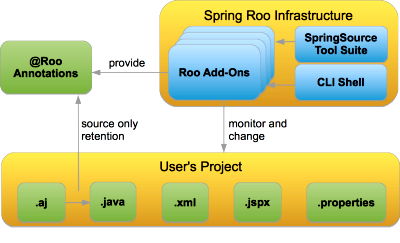
\includegraphics[scale=0.8]{img/roo-architektura.png}
    \caption{Schéma fungování Spring Roo nad projektem\cite{RooPDF}}
\end{figure}
\\
Spring Roo ve formě jednotlivých modulů - addonů (buď jako samostatný nástroj v~shell příkazové řádce, nebo jako součást balíku SpringSource Tool Suite) vytváří a sleduje změny v~uživatelských souborech, přidává anotace začínající na \textit{@Roo} do kódu a udržuje tak vazbu mezi java třídami (\textit{.java}) a deklaracemi AspectJ (\textit{.aj}).\\

\subsection{Odstranění z~projektu}
Existují rizika, kvůli kterým může vývojář chtít přestat Roo používat – např. se změní požadavky, objeví se vhodnější alternativa, nástroj může obsahovat neúnosné množství chyb, nemusí podporovat potřebné verze softwaru atd. V tom případě je velkou výhodou fakt, že Spring Roo nijak neovlivňuje běh vznikající aplikace a je ho tedy možné \uv{beztrestně} odstranit. Běh aplikace se tím nijak neovlivní. Veškerá funkcionalita Roo je využívána během vývoje a sestavené aplikace se nijak nedotýká - anotace @Roo slouží pouze k~udržování informací o~zdrojovém kódu a při kompilaci jsou odstraněny. Proto Roo nemá vliv~ani na výkon a paměťové nároky výsledného systému.\\
Odstranění Roo trvá několik minut a zahrnuje pouze refaktorování kódu a jednoduché vyhledání a nahrazení klíčových slov. Celý proces je popsán v~dokumentaci\cite{RemovingRoo} a existuje k~němu mnoho demonstrací.\\
Díky snadnému odstranění nástroje z~projektu nedochází ani k~proprietárnímu uzamčení, tedy vytvoření závislosti na jednom konkrétním nástroji nebo společnosti.

\subsection{Použitelnost}
Nástroj Spring Roo je většinou spouštěn ve zvláštním okně mimo používané IDE\footnote{Integrated Development Environment} nebo textový editor a nevyžaduje pozornost ze strany uživatele. Místo toho běží na pozadí a monitoruje změny v~projektu. Ani změny, provedené v~době, kdy Roo neběží, nejsou problémem, protože Roo při každém spuštění projde všechny soubory a případné změny vyhledá.\\
Nástroj klade velký důraz na použitelnost a jeho uživatelské rozhraní (příkazový řádek) je inspirováno knihou Jefa Raskina \textit{The Humane Interface}. Podle zásad v~ní popsaných se snaží neomezovat uživatele v~tom, co chce zrovna udělat, a nenarušovat jeho soustředění, ale naopak předvídat akce z~jeho strany a korektně na ně reagovat.\cite{Roo}\\
Roo se také snaží o~to, aby byla doba potřebná k~naučení se práce s~ním co možná nejkratší. Toho dosahuje několika způsoby:
\begin{itemize}
\item používá standardní Java technologie, u~kterých je vysoká šance, že je uživatel již zná,
\item běží na pozadí a nevyžaduje pozornost uživatele, pokud to sám nepotřebuje zadávat příkazy a provádět změny,
\item zahrnuje funkce usnadňující učení, jako je doplňování příkazů po stisknutí tabulátoru nebo kontextová nápověda ve formě příkazu \uv{hint}, který na základě stavu projektu a nedávné aktivity uživatele navrhuje další možný postup,
\item řídí se jasně definovanými konvencemi\cite{Roo-konvence},
\item pracuje v~\uv{bezpečném režimu}, takže se všechny změny provedené pomocí něj dají zvrátit díky automatickému roll-backu.
\end{itemize}

\subsection{AspectJ}
\begin{figure}[h!]
  \centering
    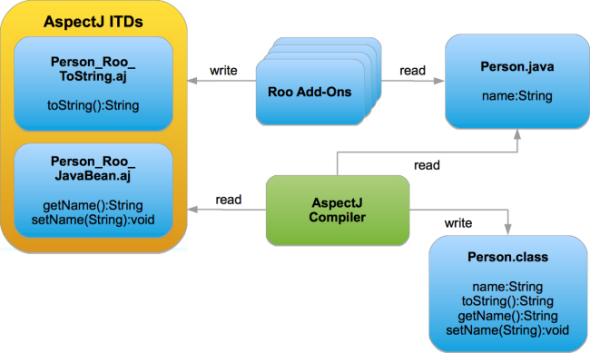
\includegraphics[scale=0.6]{img/roo-aspectj.png}
    \caption{AspectJ ITD\cite{RooPDF}}
\end{figure}

Jak se u~Springového nástroje dá očekávat\cite{Roo-AspectJ}, i~Spring Roo je z~velké části založen na technologii AspectJ – konkrétně na výhodách plynoucích z~možností ITD\footnote{Inner Type Declaration}. Metody, které generuje a spravuje Roo, nejsou obsažené přímo ve zdrojových \textit{.java} souborech, ale v~externích souborech ITD s~příponou \textit{*\string_Roo\string_*.aj}.
Ze zdrojových souborů se na tyto třídy odkazuje pouze pomocí anotací začínajících na \uv{@Roo}, které je v~případě potřeby snadné odstranit.

Příklad vytvoření třídy s~názvem \textit{Hello} pomocí Roo: 
\begin{lstlisting}[language=bash,caption=Vytvoření třídy v~Roo]
roo> project --topLevelPackage com.aspectj.rocks
roo> jpa setup --database HYPERSONIC_IN_MEMORY --provider HIBERNATE
roo> entity jpa --class ~.Hello
Created SRC_MAIN_JAVA/com/aspectj/rocks
Created SRC_MAIN_JAVA/com/aspectj/rocks/Hello.java
Created SRC_MAIN_JAVA/com/aspectj/rocks/Hello_Roo_JpaActiveRecord.aj
Created SRC_MAIN_JAVA/com/aspectj/rocks/Hello_Roo_JpaEntity.aj
Created SRC_MAIN_JAVA/com/aspectj/rocks/Hello_Roo_ToString.aj
Created SRC_MAIN_JAVA/com/aspectj/rocks/Hello_Roo_Configurable.aj
roo> field string --fieldName comment
Managed SRC_MAIN_JAVA/com/aspectj/rocks/Hello.java
Managed SRC_MAIN_JAVA/com/aspectj/rocks/Hello_Roo_JavaBean.aj
Managed SRC_MAIN_JAVA/com/aspectj/rocks/Hello_Roo_ToString.aj
\end{lstlisting}

Z výpisu konzole je vidět, že se zároveň se zdrojovým souborem \textit{Hello.java} bylo vytvořeno i~několik souborů s~názvy ve tvaru \textit{*\string_Roo\string_*.aj}.
Na zdrojovém java souboru není nic zvláštního, kromě standardního kódu obsahuje pouze několik anotací ve tvaru \textit{@Roo*}, které odkazují na metody spravované nástrojem Roo:

\begin{lstlisting}[language=Java,caption=Hello.java]
package com.aspectj.rocks;

import org.springframework.roo.addon.javabean.RooJavaBean;
import org.springframework.roo.addon.tostring.RooToString;
import org.springframework.roo.addon.entity.RooJpaActiveRecord;

@RooJavaBean
@RooToString
@RooJpaActiveRecord
public class Hello {

    private String comment;
}
\end{lstlisting}

Kód vytvořených ITD tříd se v~mnohém podobá klasické Javě. Hlavní rozdíl je v~tom, že jsou deklarované pomocí klíčových slov \textit{privileged aspect}, a~v~tom, že každá položka navíc obsahuje identifikátor určující, ke které třídě patří. V následujícím případě je tímto identifikátorem text \textit{Hello.toString}, což znamená \uv{metoda toString třídy Hello}.

\begin{lstlisting}[language=AspectJ,caption=Hello\string_Roo\string_ToString.aj]
package com.aspectj.rocks;

import java.lang.String;

privileged aspect Hello_Roo_ToString {
    
    public String Hello.toString() {    
        StringBuilder sb = new StringBuilder();        
        sb.append("Id: ").append(getId()).append(", ");        
        sb.append("Version: ").append(getVersion()).append(", ");        
        sb.append("Comment: ").append(getComment());        
        return sb.toString();        
    }    
    
}
\end{lstlisting}

Uživatel by do souborů ITD neměl nikdy zasahovat, celý jejich životní cyklus řídí Roo - automaticky je aktualizuje a~upravuje na základě uživatelských změn v~souborech \textit{.java}. Klasické zdrojové soubory nejsou nijak ovlivněny, protože metody vytvořené v~souborech \textit{.aj} se projevují až v~okamžiku kompilace a~přidávají se jako klasické Java metody do výsledných  souborů \textit{.class}.\\
Roo neustále sleduje změny ve zdrojových Java souborech a~promítá je do automaticky spravovaných souborů ITD. Pokud by například uživatel přidal metodu toString do souboru \textit{Hello.java}, Roo smaže soubor \textit{Hello\string_Roo\string_ToString.aj}, který už není k~ničemu potřeba. V případě, že uživatel změní rozhodnutí a~svou metodu odstraní, Roo příslušný soubor ITD opět vygeneruje.\\
Kompilátor tyto ITD díky anotacím rozpozná a~vloží příslušné položky do výsledných souborů \textit{.class}, jak je vidět na následujícím příkladu výpisu zkompilované třídy \textit{Hello.class}.

\begin{lstlisting}[language=bash,caption=Výpis třídy Hello]
$ mvn compile
$ javap -classpath target/classes/.:target/test-classes/. com.aspectj.rocks.Hello
Compiled from "Hello.java"
public class com.aspectj.rocks.Hello extends java.lang.Object implements org.springframework.beans.factory.aspectj.ConfigurableObject{
    transient javax.persistence.EntityManager entityManager;
    public com.aspectj.rocks.Hello();
    public static java.lang.String ajc$get$comment(com.aspectj.rocks.Hello);
    public static void ajc$set$comment(com.aspectj.rocks.Hello, java.lang.String);
    public static java.lang.Long ajc$get$id(com.aspectj.rocks.Hello);
    public static void ajc$set$id(com.aspectj.rocks.Hello, java.lang.Long);
    public static java.lang.Integer ajc$get$version(com.aspectj.rocks.Hello);
    public static void ajc$set$version(com.aspectj.rocks.Hello, java.lang.Integer);
    static {};
    public static long countHelloes();
    public static final javax.persistence.EntityManager entityManager();
    public static java.util.List findAllHelloes();
    public static com.aspectj.rocks.Hello findHello(java.lang.Long);
    public static java.util.List findHelloEntries(int, int);
    public void flush();
    public java.lang.String getComment();
    public java.lang.Long getId();
    public java.lang.Integer getVersion();
    public com.aspectj.rocks.Hello merge();
    public void persist();
    public void remove();
    public void setComment(java.lang.String);
    public void setId(java.lang.Long);
    public void setVersion(java.lang.Integer);
    public java.lang.String toString();
}
\end{lstlisting}

\subsection{Rozšíření}
Spring Roo je vysoce modulární a~využívá systém rozšíření pomocí tzv. addonů založených na platformě OSGi\cite{roo-architektura}. Každý addon reprezentuje určitou funkcionalitu, například logování pomocí knihovny Log4J nebo automatické generování testů. Jádro nástroje představuje několik základních addonů, které jsou součástí základní instalace a~poskytují klíčovou funkcionalitu, například správu potřebných knihoven, podporu JPA, nebo správu Java tříd a~základních metod.\cite{Roo-base-addons} Všechny další funkce jsou k~Roo přidávány zvlášť jako rozšíření. Díky tomu není třeba se zatěžovat technologiemi, které vývojář nechce použít, a~je snadné tyto technologie měnit a~vybírat.\\
\\
Roo umožňuje uživatelům tvorbu 4 různých typů addonů v~závislosti na jejich funkcionalitě:
\begin{enumerate}
\item \textbf{Simple}\\
Jednoduchý addon, který dokáže přidat závislosti do souboru \textit{pom.xml} a/nebo spravovat konfigurační prvky
\item \textbf{Advanced}\\
Plný addon - dokáže mj. přidávat do projektu novou funkcionalitu, přidávat nové Java typy a~ITD
\item \textbf{i18n}\\
Přidává podporu pro určitý jazyk do struktury rámce Spring MVC
\item \textbf{Wrapper}\\
Zabalí určitou knihovnu (ve formě \uv{maven artifact}) pomocí manifestu tak, aby splňoval standard OSGi\cite{osgi}. Nejčastěji se používá pro vytvoření balíku s~JDBC\footnote{Java Database Connectivity} ovladačem\cite{IBM-tutorial}.
\end{enumerate}

\section{Srovnání}
Nástroje JBoss Forge a~Spring Roo jsou v~mnoha ohledech velmi podobné. Řeší podobné oblasti, tedy významně zvyšuje produktivitu vývojářů při psaní podnikových aplikací v~jazyce Java.\\
Oba nástroje umožňují vygenerovat velké množství kódu a~nakonfigurovat v~projektu potřebné rámce a~technologie. Usnadňují práci hlavně v~začátku vývoje, protože vývojáři díky nim nemusí ani vymýšlet vlastní řešení, ani se učit nová existující řešení a~hledat příklady jejich použití a~konfigurací. Stačí zadat příkaz a~daná technologie je automaticky přidána a~nakonfigurována podle potřeby.\\
Oba nástroje jsou vydávány pod open-source licencemi, mají textové rozhraní v~příkazové řádce, poskytují uživateli kontextové doplňování příkazů a~dají se snadno integrovat do nejrozšířenějších vývojových prostředích.\\
Přestože jsou v~mnoha ale aspektech srovnatelné, existuje mezi nimi několik rozdílů. Kromě zřejmého rozdílu, tedy že Roo je nástroj více orientovaný na rámec Spring, zatímco Forge je, co se technologií týče, více agnostický, je asi největším z~nich fakt, že Roo není pouze nástroj na generování kódu, ale spíš programovací rámec, který prostřednictvím technologie AspectJ spravuje \uv{své} soubory v~průběhu celého vývoje a~průběžně je upravuje.
To může být velká výhoda, ale zvlášť ve složitějších projektech se může stát překážkou příliš velké množství vygenerovaných souborů ITD. To je problémem zvlášť v~případech, kdy na projektu pracuje zároveň více vývojářů a~využívá se nějaký verzovací systém, protože může snadno docházet ke konfliktům, které vývoj brzdí. AspectJ navíc může způsobovat problémy v~některých IDE, protože nejde o~standardní Java technologii a~vytvářené třídy jsou kompletní až ve chvíli sestavování výsledného balíku.\\
Proto je často lepší, když použije Roo na počátku projektu jeden z~vývojářů, vytvoří s~pomocí něj co možná nejvíc kódu, a~potom jej z~projektu odstraní.\cite{OpenSlava}\\
Forge se naproti tomu drží pouze Javy a~neposkytuje žádnou průběžnou podporu. Zároveň se ale snáze používá nad již existujícími projekty, protože nevyžaduje žádnou speciální nestandardní strukturu, ani jím vytvořený kód neobsahuje žádné speciální anotace, které by se odlišovaly od standardního kódu v~Javě.\cite{OpenSlava}
\\
K oběma nástrojům existuje poměrně kvalitní dokumentace. Ta je v~případě Forge je hodně praktická a~už od úvodní stránky nabízí rychlé návody k~instalaci, návody a~názorné příklady vytváření aplikací. Přibližně polovina dokumentace Forge se věnuje uživatelským rozšířením, opět formou názorného návodu, který uživatele celým procesem provede krok po kroku.
Dokumentace Forge není příliš obsáhlá a~dá se v~ní snadno vyznat, na druhou stranu ale trochu chybí úvod nebo obecný popis nástroje, jeho výhod a~mechanismů, na kterých pracuje, a~bližší technologií využívaných při tvorbě pluginů. Hodilo by se alespoň popsat možnosti a~metody existujících faset.\\
Dokumentace Spring Roo je oproti tomu velmi rozsáhlá, ale zároveň dobře strukturovaná. Popisuje Roo obecně včetně jeho vnitřního fungovaní a~výhod plynoucích z~jeho využívání. Poskytuje podrobné popisy jednotlivých aspektů tohoto nástroje i~návody a~tutoriály pro použití v~praxi. Ovšem ani dokumentace Roo není dokonalá, protože například v~části, která se věnuje tvorbě plnohodnotných addonů, text úplně chybí.\cite{Roo-advanced-addons}\\
Roo se také, na rozdíl od Forge, věnuje obsáhlý článek na webu \url{http://www.wikipedia.org/}\cite{roo-wiki}. Forge se na wikipedii zatím najít nedá a~to ani v~seznamu RAD nástrojů\cite{rad-wiki} nebo v~seznamu projektů JBoss\cite{jboss-wiki}.\\
Roo klade o~něco větší důraz na použitelnost, což je znát například na výše zmiňované funkci \textit{hint}, která vývojáře provází tvorbou aplikace a~navrhuje další postup.

\chapter{Selenium}
Selenium je sada nástrojů, která umožňuje programové ovládání webového prohlížeče. Primárně slouží k~automatickému testování webových aplikací, ale obecně ji lze použít k~libovolné činnosti spojené s~automatizací webového prohlížeče.\cite{SeleniumHQ} \\
Selenium se skládá z~několika komponent:

\section{Selenium Remote Control}

\begin{figure}[h!]
  \centering
    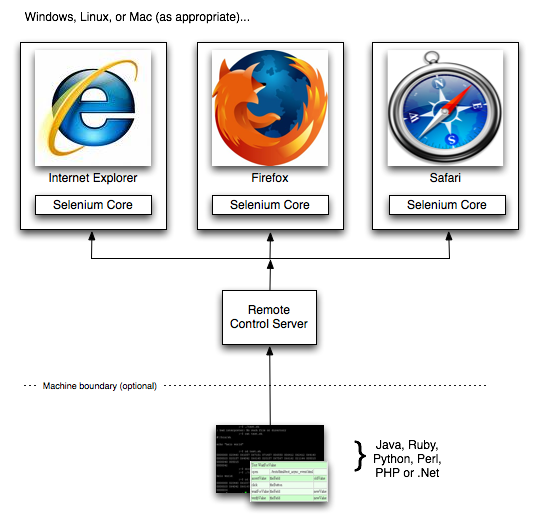
\includegraphics[scale=0.4]{img/selenium-rc.png}
    \caption{Architektura Selenium RC\cite{SeleniumRC}}
\end{figure}

Selenium RC nebo také Selenium 1 je testovací nástroj pro psaní automatických testů uživatelských rozhraní webových aplikací. Sestává ze 2 částí - serveru a~klientské knihovny. Selenium server spouští a~vypíná prohlížeč, interpretuje a~spouští příkazy v~jazyce Selenese a~přijímá HTTP GET/POST metody, klientská knihovna slouží jako rozhraní mezi používaným programovacím jazykem a~serverem Selenium.
Samotný server Selenium před spuštěném testu vloží prostřednictvím rozhraní do prohlížeče funkce v~jazyce Javascript, které potom používá k~jeho ovládání. Funguje tedy shodně pro všechny prohlížeče.\cite{SeleniumRC}\\

Selenium RC je v~současné době stále aktivně podporován, ale dále se nerozvíjí a~byl oficiálně označen jako \uv{deprecated}. Jeho nástupcem je projekt Selenium 2 (WebDriver).\cite{Selenium-history}

\section{Selenium Grid}
Selenium Grid umožňuje škálování testů (pro Selenium RC i~WebDriver) prostřednictvím jejich paralelního spouštění na několika počítačích a~prohlížečích zároveň.
Umožňuje správu paralelních běhů z~jednoho místa, testy se tak dají spouštět zároveň na kombinacích různých operačních systémů a~prohlížečů.\cite{Selenium-Grid}

\section{Selenium WebDriver}
Selenium Webdriver (nebo Selenium 2) je projekt, který nahrazuje systém Selenium RC. Jedná se o~sadu API specifických a~zvlášť upravených pro každý prohlížeč. Na rozdíl od Selenia RC WebDriver spouští a~ovládá přímo samotný prohlížeč pomocí jeho nativních metod přesně tak, jak by ho ovládal uživatel. Není proto třeba (až na výjimečné případy - například ve spojení s~nástrojem Selenium Grid) používat Selenium-Server, na druhou stranu musí mít každý prohlížeč svou vlastní implementaci ovladače.\cite{webdriver-dokumentace}\\
WebDriver poskytuje pro jednotlivé prohlížeče objektově orientované rozhraní, které pohlíží na prohlížeč jako objekt a~umožňuje volat jeho metody, vyhledávat jeho elementy atd. Tím se výrazně zjednodušuje psaní testů. V současné době existují následující ovladače prohlížečů: AndroidDriver, ChromeDriver, EventFiringWebDriver, FirefoxDriver, HtmlUnitDriver, InternetExplorerDriver, IPhoneDriver, PhantomJSDriver, RemoteWebDriver a~SafariDriver.\cite{WebDriver-drivery}\\
Rozhraní WebDriver se postupně stává internetovým standardem konsorcia W3C.\cite{WebDriver-W3C}

\section{Arquillian}
Arquillian je testovací rámec, který mimo jiné podporuje testování webových aplikací. K tomu slouží především 2 rozšíření tohoto systému - Arquillian Drone a~Arquillian Graphene 2, která se navzájem velmi dobře spolupracují a~hodí se pro účely RAD vývoje.

\subsection{Arquillian Drone}
Arquillian Drone je rozšíření, které do testovacího rámce Arquillian přidává podporu technologie Selenium. Pro účely testování webových aplikací a~RAD vývoje přináší zejména výhody v~těchto 3 oblastech: 

\begin{enumerate}
\item konfigurace - umožňuje vyčlenit veškerou konfiguraci přehledně do jednoho souboru mimo samotný kód testu,
\item správa životního cyklu prohlížeče - jeho relace navíc není po skončení testu uzavřena, ale je znovu využívána pro další testy místo toho, místo toho, aby se pro každý test spouštěla zvláštní instance prohlížeče. Díky tomu je testování výrazně urychleno.
\item interakce s~nasazením a~kontejnery poskytovanými systémem Arquillian - aplikace je automaticky nasazena na server pomocí metody \textit{\@Deployment} bez potřeby ručního zásahu vývojáře\cite{ArqDrone}
\end{enumerate}

\subsection{Arquillian Graphene 2}
Arquillian Graphene funguje jako rozšíření rozhraní WebDriver a~zaměřuje se na rychlý vývoj a~použitelnost v~prostředí programovacího jazyka Java. 
Testy psané přímo pro WebDriver jsou poměrně úzce spjaté s~HTML strukturou testovaných stránek. Tato struktura se ale v~průběhu vývoje často mění, což může testy negativně ovlivnit. Arquillian Graphene poskytuje abstrakci nad testovanými stránkami a~pomocí mechanismů nazvaných \textit{Page Objects} a~\textit{Page Fragments} odděluje testy od struktury testovaných webových stránek. Tím se zvyšuje jejich robustnost, přehlednost a~znovupoužitelnost.\cite{Graphene}

\chapter{Implementace rozšíření}
Pro účely porovnání rozšiřitelnosti nástrojů Spring Roo a~JBoss Forge bylo pro každý z~nich vytvořeno vzorové rozšíření.
Tato rozšíření umožňují automaticky generovat testy webového rozhraní, které využívají technologie WebDriver a~JUnit.
Obě řešení používají prohlížeč Mozilla Firefox, jehož relace je testu inicializována a~ukončena pomocí standardních anotací testovacího rámce JUnit: 

\begin{lstlisting}[language=Java,caption=Hello.java]
private WebDriver driver;

    @Before
    public void setUp() {
        driver = new FirefoxDriver();
        driver.manage().timeouts().implicitlyWait(5, TimeUnit.SECONDS);
    }

    @Test
    public void test() {
       ...
    }

    @After
    public void tearDown() {
        driver.quit();
    }
\end{lstlisting}    

Nová rozšíření nevytvářejí kompletní testy, protože jejich podoba do jisté míry závisí na technologii použité při tvorbě prezentační vrstvy. Místo toho vytvářejí kostru testů s~názornými příklady použití rozhraní WebDriver a~odkazy na jeho dokumentaci.

\section{Plugin pro JBoss Forge}
Tvorba rozšíření pro JBoss Forge začíná vytvořením prázdného projektu se strukturou Maven. Příkaz \textit{plugins setup} přidá potřebné závislosti rozhraní Forge Plugin API a~příkaz \textit{plugins new-plugin} vytvoří jednoduchou třídu, která implementuje rozhraní \textit{org.jboss.forge.shell.plugins.Plugin} a~která názorně demonstruje práci s~příkazy a~jejich parametry.\\
\\
Jako předloha pro rozšíření nástroje JBoss Forge sloužil existující plugin \textit{plugin-arquillian}\cite{plugin-arquillian}, který umožňuje automatické generování testů využívajících testovací rámec Arquillian. \\
Nově vytvořený plugin umožňuje využívat dva příkazy. První z~nich, příkaz \textit{add-dependencies}, přidává do souboru \textit{pom.xml} potřebné závislosti, druhý příkaz potom generuje vlastní test pro třídu, kterou uživatel určí v~parametru.\\
JBoss Forge se při zavolání příkazu \textit{add-dependencies} připojí k~repozitáři systému Maven a~vybídne uživatele k~výběru verze dané knihovny ze seznamu všech dostupných verzí.\\
Podobně jako plugin \textit{plugin-arquillian}, i~nové rozšíření využívá pro generování testů šablonu ve formátu Apache Velocity\cite{velocity}, která umožňuje snadno operovat s~objekty jazyka Java. To je názorně vidět na následujícím příkladu:

\begin{lstlisting}[language=Java,caption=Příklad zpřístupnění objektů v~šabloně]
	VelocityContext context = new VelocityContext();
    context.put("package", javaSource.getPackage());
    context.put("ClassToTest", javaSource.getName());
    context.put("classToTest", javaSource.getName().toLowerCase());
    context.put("packageImport", javaSource.getPackage());
    context.put("fields", fields);
    context.put("projectName", metaData.getProjectName());

    StringWriter writer = new StringWriter();
    Velocity.mergeTemplate("TestTemplate.vtl", "UTF-8", context, writer);

    JavaClass testClass = JavaParser.parse(JavaClass.class, writer.toString());
    java.saveTestJavaSource(testClass);
\end{lstlisting}         
        
\begin{lstlisting}[language=Java,caption=Používání java objektů v~šabloně testu]        
	driver.get(baseUrl + indexPage);
    driver.findElement(By.linkText("${ClassToTest}")).click();
    driver.findElement(By.linkText("Create New")).click(); 
\end{lstlisting}            
        
\subsection{Arquillian}                
Na přání vedoucího práce byl vyvinut i~druhý plugin pro JBoss Forge, který navíc využívá výše zmíněné technologie Arquillian Drone a~Arquillian Graphene 2. Tento plugin mj. vytváří vzorový konfigurační soubor \textit{arquillian.xml} a~umožňuje konfiguraci testů, například výběr použitého prohlížeče.\\
V samotných generovaných testech využívá metodu s~anotací \textit{\@Deployment}, díky které je aplikace před spuštěním testu automaticky sestavena pomocí mechanismu ShrinkWrap\cite{shrinkwrap} a~nasazena na server. Je zde také využit systém abstrakcí stránek poskytovaný technologií Arquillian Graphene 2.\\
Tento druhý plugin představuje pro praxi asi nejpřínosnější výstup práce, protože je uživatelsky mnohem přívětivější a~lépe odpovídá prostředí nástroje JBoss Forge a~principům RAD.
Zbylá dvě rozšíření byla vytvořena spíš za účelem demonstrování rozšiřitelnosti obou porovnávaných platforem.

\section{Addon pro Spring Roo}
Spring Roo nabízí čtyři typy rozšíření, z~nichž se pro účely této práce nejlépe hodí typ \textit{advanced addon}, který umožňuje mj. vytvářet nové Java třídy.\\
Tvorba addonu začíná voláním příkazu \textit{addon create advanced}. Tím je vytvořena struktura addonu a~ukázkový kód, který demonstruje práci se soubory ITD a~anotacemi. Správa tříd ITD je řešena pomocí systému tzv. \uv{listenerů} a~reagování na události platformy OSGi, což zahrnuje kód na poměrně nízké úrovni.\\
\\
Jako předloha pro nový addon byly použity existující addony \textit{addon-test}\cite{addon-test} a~\textit{addon-web-selenium}\cite{addon-web-selenium}, které umožňují generovat integrační ukázkové testy resp. vytváří Selenium testy ve formátu Selenese\cite{selenese}.\\
Podobně jako plugin pro JBoss Forge, i~toto rozšíření zahrnuje dva příkazy - jeden k~instalaci závislostí a~druhý k~vlastnímu generování testů.\\
V případě Roo jsou potřebné závislosti definovány v~konfiguračním souboru \textit{configuration.xml}, ze kterého se pouze překopírují do souboru \textit{pom.xml} cílového projektu. Toto řešení je sice o~trochu snadnější, než v~případě Forge, na druhou stranu uživatel nemůže během instalace závislostí volit jejich verze, které se s~časem mění.\\
I struktura generovaného testu je stejná, jako v~případě pluginu pro Forge, jeho generování však není řešeno pomocí šablony, ale probíhá pomocí sady tzv. \uv{builderů}, tedy objektů, které výslednou třídu sestavují. Tento přístup je o~něco flexibilnější a~nabízí více možností, na druhou stranu je k~dosažení podobného výsledku potřeba mnohem více kódu, který je navíc poměrně nepřehledný.

\begin{lstlisting}[language=Java,caption=Sestavení metody pomocí třídy MethodMetadataBuilder]
private MethodMetadataBuilder getBeforeMethod(String declaredByMetadataId, JavaType controller) {
		final InvocableMemberBodyBuilder bodyBuilderBefore = new InvocableMemberBodyBuilder();				
		final List<AnnotationMetadataBuilder> methodAnnotationsBefore = new ArrayList<AnnotationMetadataBuilder>();
		methodAnnotationsBefore.add(new AnnotationMetadataBuilder(BEFORE));
		final MethodMetadataBuilder methodBuilderBefore = new MethodMetadataBuilder(
				declaredByMetadataId, Modifier.PUBLIC, new JavaSymbolName(
						"setUp"), JavaType.VOID_PRIMITIVE, bodyBuilderBefore);
		methodBuilderBefore.setAnnotations(methodAnnotationsBefore);
		return methodBuilderBefore;
	}	
\end{lstlisting}

\section{Srovnání}
Z hlediska rozšiřitelnosti jsou rozdíly mezi Forge a~Roo patrné ještě dříve, než člověk začne vůbec psát kód. Zatímco Forge v~novém projektu vytvoří jednu přehlednou třídu s~přibližně 50 řádky kódu, Roo vytvoří skoro desetkrát více kódu v~celkem pěti třídách a~jednom konfiguračním souboru. Přesto, že je v~nově vygenerovaném projektu hodně komentářů, není snadné se v~něm vyznat.\\
Samotná implementace nových rozšíření je o~něco jednodušší v~případě Forge, opět kvůli tomu, že jeho rozhraní nabízí v~porovnání s~Roo o~něco vyšší úroveň abstrakce, a~proto je výsledný kód úspornější a~přehlednější. Pro Forge navíc existuje více tutoriálů.\\
Stejně tak lokální instalace nových rozšíření z~lokálních souborů je snadnější v~případě JBoss Forge, protože stačí tento nástroj jedním příkazem nasměrovat do adresáře s~projektem. O sestavení a~instalaci pluginu se postará sám.\\
Při instalaci addonů Roo je potřeba nový addon nejprve sestavit příkazem \textit{perform assembly} a~poté výsledný \textit{.jas} soubor nainstalovat pomocí příkazu pro platformu OSGi. Pokud jde o~opakovanou instalaci například během vývoje, je navíc třeba starší verzi addonu nejprve ručně odinstalovat.\\
Tvorba nových rozšíření se podle mého názoru spíše vyplatí v~případě Forge, protože mnohem více splňuje principy RAD. I~zde ale existují místa, která se dají vylepšit - například málo popisná dokumentace.\\
Naproti tomu vytváření nových addonů pro Roo může zejména nezkušené vývojáře odradit množstvím poměrně složitého kódu a~neúplností dokumentace.\\
Přestože jsou srovnávané nástroje v~mnoha ohledech velmi podobné, v~otázce snadnosti vývoje uživatelských rozšíření jednoznačně vede JBoss Forge. 
    
\chapter{Závěr}
Zadáním této bakalářské práce bylo zmapovat současný stav RAD nástrojů Spring Roo a~JBoss Forge, vytvořit pro každý z~nich rozšíření se shodnou funkcionalitou a~na základě zjištěných informací nástroje porovnat. Při výsledném porovnání se klade důraz na rozšiřitelnost zkoumaných nástrojů.\\
Jako téma vytvářených rozšíření bylo zvoleno generování testů rozhraní webových aplikací s~využitím technologie WebDriver. Rozšíření s~touto funkcionalitou dříve ani pro jeden z~těchto nástrojů neexistovalo.\\
Mimo rozsah této práce navíc vzniklo druhé rozšíření pro JBoss Forge s~podobnou funkcionalitou, které je uživatelsky přívětivější díky využití technologií Arquillian Drone a~Arquillian Graphene 2. Toto řešení bude navrženo k~zařazení do CPI.

\section*{Další rozvoj}
Rozšíření pro Spring Roo by bylo vhodné dále rozvinout podle návrhů popsaných v~systému Jira\cite{roo-jira} projektu Spring Roo.

%% Lists of tables and figures, glossary, etc.
\listoffigures

\begin{thebibliography}{13}

\bibitem{Roo}
ALEX, Ben, Stefan SCHMIDT, Alan STEWART, James TYRRELL a Andrew SWAN. SPRING. \textit{Spring Roo - Reference Documentation} [online]. 1.2.4.RELEASE. 2013 [cit. 2013-12-04]. Dostupné~z:
\url{http://docs.spring.io/spring-roo/reference/html/}.

\bibitem{SeleniumHQ}
OPENQA. \textit{Selenium} [online]. 2013 [cit. 2013-12-07]. Dostupné~z:
\url{http://www.seleniumhq.org/}.

\bibitem{SeleniumRC}
OPENQA. \textit{Selenium 1 (Selenium RC)} [online]. 2013 [cit. 2013-12-07]. Dostupné~z:
\url{http://www.seleniumhq.org/docs/05_selenium_rc.jsp}.

\bibitem{ArqDrone}
JBOSS. \textit{Arquillian Drone} [online]. 2013 [cit. 2013-12-07]. Dostupné~z:
\url{https://docs.jboss.org/author/display/ARQ/Drone}

\bibitem{Forge}
JBOSS. \textit{JBoss Forge} [online]. 2013 [cit. 2013-12-07]. Dostupné~z:
\url{http://forge.jboss.org/docs/}

\bibitem{BlueInk}
BLUE INK. \textit{Rapid Application Development} [online]. 2005 [cit. 2013-12-17]. Dostupné~z:
\url{http://www.blueink.biz/RapidApplicationDevelopment.aspx}

\bibitem{RooPDF}
SCHMIDT, Stefan. BLUE INK. \textit{Spring Roo:Open-Source Rapid Application Development for Java} [online]. 2012 [cit. 2013-12-20]. Dostupné~z:
\url{http://refcardz.dzone.com/refcardz/spring-roo-open-source-rapid}

\bibitem{RemovingRoo}
ALEX, Ben, Stefan SCHMIDT, Alan STEWART, James TYRRELL a Andrew SWAN. SPRING. \textit{Spring Roo - Reference Documentation: Chapter 6. Removing Roo} [online]. 2013 [cit. 2013-12-27]. Dostupné~z:
\url{http://docs.spring.io/spring-roo/reference/html/removing.html}

\bibitem{Roo-konvence}
ALEX, Ben, Stefan SCHMIDT, Alan STEWART, James TYRRELL a Andrew SWAN. SPRING. \textit{Spring Roo - Reference Documentation: Chapter 4. Usage and Conventions} [online]. 2013 [cit. 2013-12-27]. Dostupné~z:
\url{http://docs.spring.io/spring-roo/reference/html/usage.html}

\bibitem{Roo-base-addons}
ALEX, Ben, Stefan SCHMIDT, Alan STEWART, James TYRRELL a Andrew SWAN. SPRING. \textit{Spring Roo - Reference Documentation: Chapter 7. Base Add-On Overview} [online]. 2013 [cit. 2013-12-27]. Dostupné~z:
\url{http://docs.spring.io/spring-roo/reference/html/base-overview.html}

\bibitem{Roo-AspectJ}
ALEX, Ben, Stefan SCHMIDT, Alan STEWART, James TYRRELL a Andrew SWAN. SPRING. \textit{Spring Roo - Reference Documentation: 3.2.1. AspectJ} [online]. 2013 [cit. 2013-12-28]. Dostupné~z:
\url{http://docs.spring.io/spring-roo/reference/html/architecture.html#architecture-critical-technologies-aspectj}

\bibitem{Roo-clanek}
WÄHNER, Kai. \textit{When to use Spring Roo?} [online]. 2011 [cit. 2013-12-28]. Dostupné~z:
\url{http://java.dzone.com/articles/when-use-spring-roo}

\bibitem{OpenSlava}
TIHOMIROVS, Vladimirs. OpenSlava 2013: Java code generation. \textit{YouTube} [online]. 2013 [cit. 2013-12-29]. Dostupné~z:
\url{http://www.youtube.com/watch?v=Gme6wumCOKo}

\bibitem{Forge-blog}
BAXTER III, Lincoln. Seam Forge 1.0.0.Alpha3 "Angry Kittens" Released. In: \textit{JBoss Community} [online]. 2011 [cit. 2013-12-30]. Dostupné~z:
\url{https://community.jboss.org/people/lincolnthree/blog/2011/04/04/seam-forge-100alpha3-angry-kittens-released}

\bibitem{Rad-tools}
MOLLEMA, Gijs. Java RAD and scaffolding tools. In: \textit{IPROFS Technology Blog} [online]. 2011 [cit. 2013-12-07]. Dostupné~z:
\url{http://blog.iprofs.nl/2011/12/22/java-rad-and-scaffolding-tools/}

\bibitem{Selenium-Grid}
OPENQA. \textit{Grid2} [online]. 2013 [cit. 2013-12-30]. Dostupné~z:
\url{http://code.google.com/p/selenium/wiki/Grid2}

\bibitem{WebDriver-W3C}
STEWART, Simon a David BURNS. \textit{WebDriver: W3C Working Draft 12 March 2013} [online]. 2013 [cit. 2013-12-31]. Dostupné~z:
\url{http://www.w3.org/TR/webdriver/}

\bibitem{Graphene}
JBOSS. \textit{Arquillian Graphene 2} [online]. 2013 [cit. 2013-12-31]. Dostupné~z:
\url{https://docs.jboss.org/author/display/ARQGRA2/Home}

\bibitem{Forge-Facets}
JBOSS. \textit{Enable modular functionality with Facets} [online]. 2013 [cit. 2013-12-07]. Dostupné~z:
\url{http://forge.jboss.org/docs/plugin_development/facets.html#content}

\bibitem{Forge-CPI}
JBOSS. \textit{Add your Plugin to the Central Plugin Index (CPI)} [online]. 2013 [cit. 2013-12-31]. Dostupné~z:
\url{http://forge.jboss.org/docs/plugin_development/add-plugin-cpi.html#content}

\bibitem{Selenium-history}
OPENQA. \textit{Brief History of The Selenium Project} [online]. 2013 [cit. 2013-12-31]. Dostupné~z:
\url{http://www.seleniumhq.org/docs/01_introducing_selenium.jsp#selenium-history}

\bibitem{WebDriver-drivery}
OPENQA. \textit{Selenium-WebDriver’s Drivers} [online]. 2013 [cit. 2013-12-31]. Dostupné~z:
\url{http://www.seleniumhq.org/docs/03_webdriver.jsp#selenium-webdriver-s-drivers}

\bibitem{CDI}
\textit{What is CDI?} [online]. 2013 [cit. 2013-12-31]. Dostupné~z:
\url{http://www.cdi-spec.org/}

\bibitem{IBM-tutorial}
GULATI, Shekhar. \textit{Introducing Spring Roo, Part 5: Write advanced and wrapper Spring Roo add-ons} [online]. 2012 [cit. 2013-12-07]. Dostupné~z:
\url{http://www.ibm.com/developerworks/library/os-springroo5/}

\bibitem{Roo-advanced-addons}
ALEX, Ben, Stefan SCHMIDT, Alan STEWART, James TYRRELL a Andrew SWAN. SPRING. \textit{Spring Roo - Reference Documentation: Chapter 19. Advanced Add-Ons} [online]. 2013 [cit. 2014-01-01]. Dostupné~z:
\url{http://docs.spring.io/spring-roo/reference/html/advanced-addons.html}

\bibitem{plugin-arquillian}
Forge / plugin-arquillian. In: \textit{GitHub} [online]. 2014 [cit. 2014-01-02]. Dostupné~z:
\url{https://github.com/forge/plugin-arquillian}

\bibitem{webdriver-dokumentace}
OPENQA. \textit{Selenium WebDriver} [online]. 2013 [cit. 2014-01-02]. Dostupné~z:
\url{http://docs.seleniumhq.org/docs/03_webdriver.jsp}

\bibitem{addon-test}
Spring-projects / spring-roo. In: \textit{GitHub} [online]. 2013 [cit. 2014-01-02]. Dostupné~z:
\url{https://github.com/spring-projects/spring-roo/tree/master/addon-test}

\bibitem{addon-web-selenium}
Spring-projects / spring-roo. In: \textit{GitHub} [online]. 2013 [cit. 2014-01-02]. Dostupné~z:
\url{https://github.com/spring-projects/spring-roo/tree/master/addon-web-selenium}

\bibitem{velocity}
THE APACHE SOFTWARE FOUNDATION. \textit{What is Velocity?} [online]. 2007 [cit. 2014-01-02]. Dostupné~z:
\url{http://velocity.apache.org/engine/releases/velocity-1.5/user-guide.html#what_is_velocity}

\bibitem{selenese}
OPENQA. \textit{Selenium Commands – “Selenese”} [online]. 2013 [cit. 2014-01-02]. Dostupné~z:
\url{http://www.seleniumhq.org/docs/02_selenium_ide.jsp#selenium-commands-selenese}

\bibitem{shrinkwrap}
JBOSS. \textit{Painless Packaging for Java} [online]. 2012 [cit. 2014-01-02]. Dostupné~z:
\url{http://www.jboss.org/shrinkwrap}

\bibitem{roo-wiki}
Spring Roo In: \textit{Wikipedia: the free encyclopedia} [online]. San Francisco (CA): Wikimedia Foundation, 2001- [cit. 2014-01-02]. Dostupné~z:
\url{http://en.wikipedia.org/wiki/Spring_Roo}

\bibitem{rad-wiki}
List of graphical user interface builders and rapid application development tools. In: \textit{Wikipedia: the free encyclopedia} [online]. San Francisco (CA): Wikimedia Foundation, 2001- [cit. 2014-01-02]. Dostupné~z:
\url{http://en.wikipedia.org/wiki/List_of_graphical_user_interface_builders_and_rapid_application_development_tools}

\bibitem{jboss-wiki}
List of JBoss software In: \textit{Wikipedia: the free encyclopedia} [online]. San Francisco (CA): Wikimedia Foundation, 2001- [cit. 2014-01-02]. Dostupné~z:
\url{http://en.wikipedia.org/wiki/List_of_JBoss_software}

\bibitem{roo-jira}
Enhancements to the Roo Selenium Test Framework. In: \textit{Spring Roo: JIRA} [online]. 2012 [cit. 2014-01-02]. Dostupné~z:
\url{https://jira.springsource.org/browse/ROO-2448}

\bibitem{roo-architektura}
ALEX, Ben, Stefan SCHMIDT, Alan STEWART, James TYRRELL a Andrew SWAN. SPRING. \textit{Spring Roo - Reference Documentation: Chapter 3. Application Architecture} [online]. 2013 [cit. 2014-01-01]. Dostupné~z:
\url{http://docs.spring.io/spring-roo/reference/html/architecture.html}

\bibitem{osgi}
OSGI ALLIANCE. \textit{OSGi Alliance Specifications} [online]. 2012 [cit. 2014-01-02]. Dostupné~z:
\url{http://www.osgi.org/Specifications/HomePage}

\bibitem{Forge-prezentace}
OracleLearning: Forge New Ground in Rapid Enterprise Software Development In: \textit{YouTube} [online]. 2013 [cit. 2013-12-31]. Dostupné~z:
\url{http://www.youtube.com/watch?v=Clso5vtKu9k}

\end{thebibliography}

%% Additional materials
\appendix

%% End of the whole document
\end{document}
